\documentclass{beamer}
\usepackage{etex}
\usetheme{Antibes}
\usepackage{amssymb,amsmath,amsthm}
\usepackage{graphicx}
\usepackage{caption}
\usepackage{subfig}
%\definecolor{cardinal}{rgb}{0.77, 0.12, 0.23}
%\usecolortheme[named=cardinal]{structure}
%\setbeamercolor{block title}{bg=cardinal,fg=black}
 \usepackage{tikz}
 \usetikzlibrary{patterns,snakes,plotmarks}
 \usepackage{multirow}
% \usetikzlibrary{shadows}
\usepackage{epstopdf}
\usepackage{nicefrac}
\usepackage{lmodern}
\usepackage{pgfplots}
\usepackage{qtree}
\newcommand*{\Scale}[2][4]{\scalebox{#1}{\ensuremath{#2}}}%
\DeclareCaptionLabelSeparator{horse}{:\,\,} % change according to your needs
\captionsetup{
  labelsep = horse,
  figureposition = bottom % used to get the correct vertical space between the figure and the caption
}
\setbeamertemplate{caption}[numbered]
\setbeamertemplate{items}[circle]
\setbeamertemplate{enumerate items}[square]
\theoremstyle{definition}
\newtheorem*{exs}{Examples}
\newtheorem{ex}{Example}
\newtheorem*{exc}{Exercise}
\newcommand{\bn}{\begin{enumerate}[i)]}
\newcommand{\en}{\end{enumerate}}
\newcommand{\im}{\item}
\newcommand{\CPT}[1]{\large{\textbf{CHAPTER #1}}}
\newcommand{\ir}[1]{\textbf{Remark #1}}
\newcommand{\ith}[1]{\textbf{Theorem #1}}
\newcommand{\idf}[1]{\textbf{Definition #1}}
\newcommand{\iex}[1]{\textbf{Example #1}}

%\usepackage{booktabs}
\setlength{\parindent}{0pt}
%\setbeameroption{show notes}
 \setbeamerfont{note page}{size=\tiny}
%\setbeamertemplate{note page}[plain]
%\setbeameroption{show only notes}
\title{Math 629 - Survival Analysis \\ Chapter 1}
\author{Drew Lazar}
\institute{Ball State University}
\date{\today}

\begin{document}
\begin{frame}
    \titlepage
\end{frame}
\section{Chapter 1}
\begin{frame}\frametitle{Types of Censoring}
\bn
\item \textbf{Right Censoring:} An observation is \textbf{right censored} if the survival time is longer than its observed value. Some examples:
\bni
\item A five year study is conducted on how long it takes for machines to break down. A particular machine is observed from the start of the study but breaks down \textbf{after the study ends}.
\item Patients are followed for ten years after having a major heart attack. The response variable is time until death. A patient \textbf{withdraws} from the study after being followed for 2 years and moves to another country.
\item A study is done on smokers who have quit to see if they will resume smoking. Study participants are contacted by telephone. A participant changes his phone number, can not be reached and is \textbf{lost to follow-up}.
\en
\en
\end{frame}
\begin{frame} \frametitle{Types of Censoring cont'd}

\bn \setcounter{enumi}{2}
\item \textbf{Left Censoring:} An observation is \textbf{left censored} if the survival time is shorter than its observed value. For example, we following persons at risk until they become HIV positive.  For some patients we may not know the exact time becoming HIV, and therefore do not know exactly when the failure occurred.
\item \textbf{Interval Censoring:} An observation is \textbf{interval censored} if the event is known to occur in some interval. For example, a study is done to see the time until children can count to ten. The children are observed every 2 months. A child can count to ten at a follow-up time but couldn't count to ten at the previous visit.
\en
\end{frame}


\begin{frame}
\begin{columns}
    \begin{column}{0.48\textwidth}
        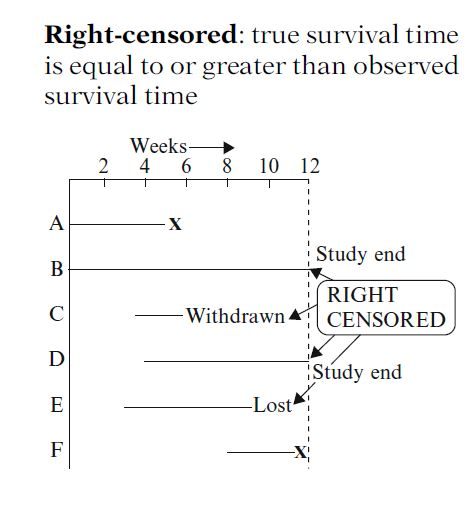
\includegraphics[width = \textwidth]{Ch1-RightCensor.JPG}
    \end{column}
    \hspace{-40pt}
    \begin{column}{0.48\textwidth}
         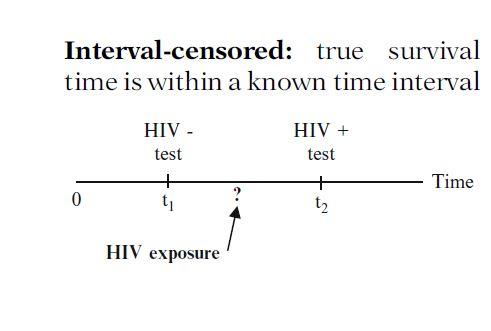
\includegraphics[width = \textwidth]{Ch1-IntervalCensor.JPG} \\
              \vspace{-20pt}
         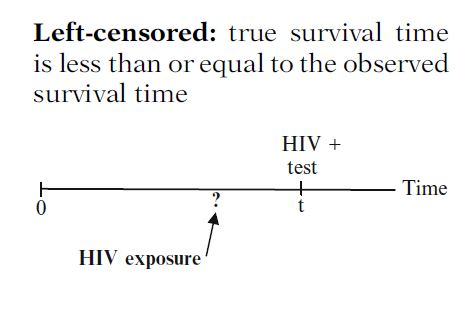
\includegraphics[width =\textwidth]{Ch1-LeftCensor.JPG}
    \end{column}
\end{columns}
\end{frame}
\begin{frame} \frametitle{Considerations about hazard rate}
\begin{block}{Hazard rate is dependent on time}
\begin{enumerate}
\item The hazard rate is dependent on the unit of measurement of time. For example, say $S$ is time measured in seconds.
\[
h(s) = \lim_{\Delta s \to 0} \frac{P(S + \Delta s|S \ge s)}{\Delta s}
\]

If say, $T$ is time measure in minutes then
\begin{align*}
h(t) & = \lim_{\Delta t \to 0} \frac{P( + \Delta t|S \ge t)}{\Delta t} \\
& = \lim_{\Delta s \to 0} \frac{P(T/60 + \Delta t/60| T/60 \ge t/60)}{ \Delta t/60} = 60 h(s)
\end{align*}

\end{enumerate}
\end{block}
\end{frame}

\begin{frame}\frametitle{Considerations about hazard rate (cont'd)}
\begin{block}{Other considerations about hazard rate}
\begin{enumerate}
  \setcounter{enumi}{1}
\item Relative rates of hazard are the same at any particular time.  For example, at any particular time (in seconds),~$s$, let $h(s,0)$ be the hazard for men (sex=0) and $h(s,1)$ be the hazard for women (sex=1). Then with $t$ the time in minutes,
    \[ \dfrac{h(t,0)}{h(t,1)} =  \dfrac{60 h(s,0)}{60 h(s,1)} = \dfrac{ h(s,0)}{ h(s,1)}
    \]
\item Can identify underlying distribution from hazard rate, for example, exponential has constant hazard, Weibull has proportional and monotonic hazard, lognormal has increasing than decreasing hazard, etc.
\item Can recover survival function from hazard rate.
\end{enumerate}
\end{block}
\end{frame}

\begin{frame}\frametitle{Hazard Functions of Different Distributions}
\begin{columns}
    \begin{column}{0.48\textwidth}
        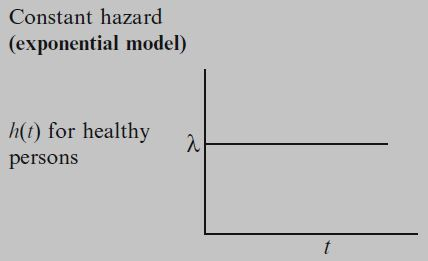
\includegraphics[width = \textwidth]{Hazards1.JPG} \\
           \includegraphics[width = \textwidth]{Hazards2.JPG}
    \end{column}
    \hspace{-10pt}
    \begin{column}{0.48\textwidth}
              \vspace{-20pt}
         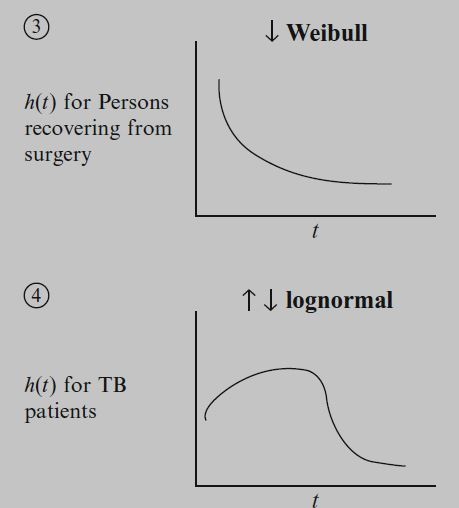
\includegraphics[width =\textwidth]{Hazards3.JPG}
    \end{column}
\end{columns}
\end{frame}



\begin{frame}
\frametitle{Ways to represent (right censored) survival data (cont'd)}
\begin{block}{First way to represent data }
\begin{columns}
    \begin{column}{0.48\textwidth}
        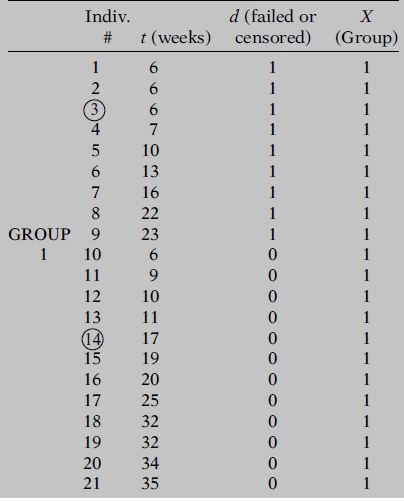
\includegraphics[width =\textwidth, height=6cm]{Ch1-leuk_dat_a.JPG}
    \end{column}
    \hspace{-10pt}
    \begin{column}{0.48\textwidth}
         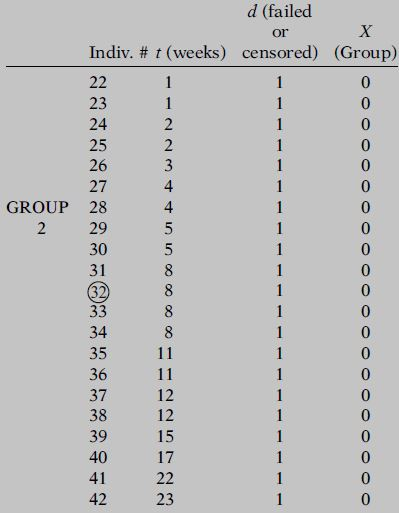
\includegraphics[width =\textwidth, height=6cm]{Ch1-leuk_dat_b.JPG}
    \end{column}
\end{columns}
\end{block}
\end{frame}

\begin{frame}
\frametitle{Ways to represent (right censored) survival data}
Consider the following data of times to remission of leukemia patients:
\begin{block}{Second way to represent data }
\begin{table}
\begin{center}
\begin{tabular}{l l}
Group 1 (n=21) treatment & Group 2 (n=22) placebo \\
 6, 6, 6, 7, 10, 13, 16, 22, 23, & 1, 1, 2, 2, 3, 4, 4, 5, 5,  \\
 6+, 19+, 20+, 25+, 32+,& 8, 8, 8, 8, 15, 17, 22, 23 \\
  32+, 34+, 35+ &
\end{tabular}
\end{center}
\end{table}
Note: + denotes censored
\end{block}
\end{frame}

\begin{frame}
\frametitle{Ways to represent (right censored) survival data (cont'd)}
\begin{block}{Third way to represent data }
\begin{columns}
    \begin{column}{0.48\textwidth}
        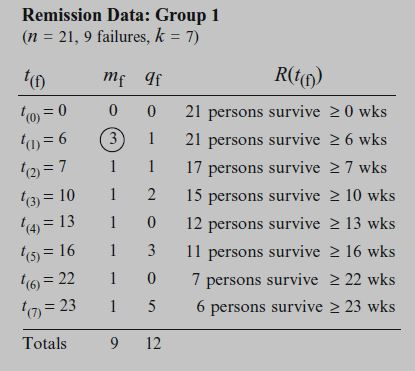
\includegraphics[width =\textwidth, height=6cm]{Ch1-leuk_data_a1.JPG}
    \end{column}
    \hspace{-10pt}
    \begin{column}{0.48\textwidth}
         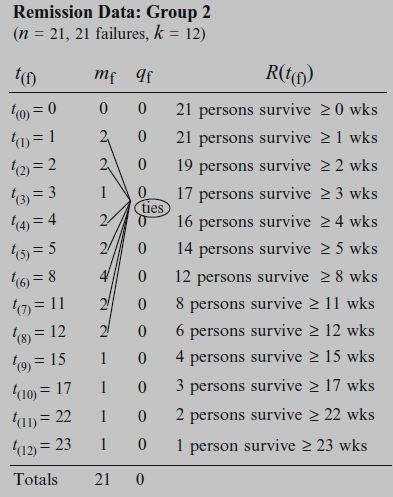
\includegraphics[width =\textwidth, height=6cm]{Ch1-leuk_data_b1.JPG}
    \end{column}
\end{columns}
\end{block}
\end{frame}

\begin{frame}
\frametitle{Ways to represent (right censored) survival data (cont'd)}
\begin{block}{Fourth way to represent data - Counting Process (CP) format}
\begin{columns}
    \begin{column}{0.48\textwidth}
        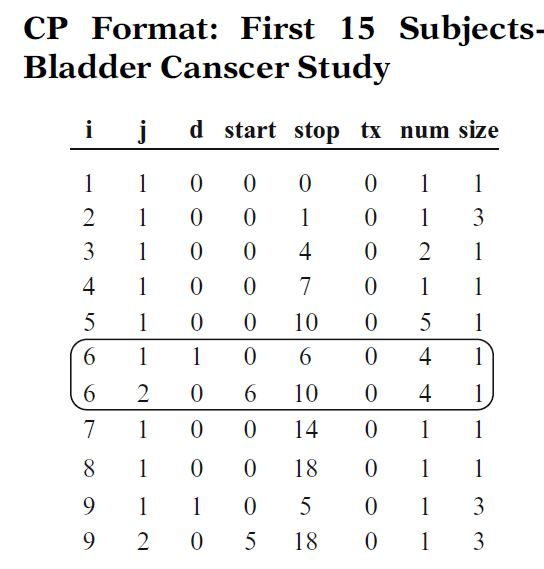
\includegraphics[width =\textwidth, height=5.5cm]{Ch1-CPFormat_1.JPG}
    \end{column}
    \hspace{-10pt}
    \begin{column}{0.48\textwidth}
         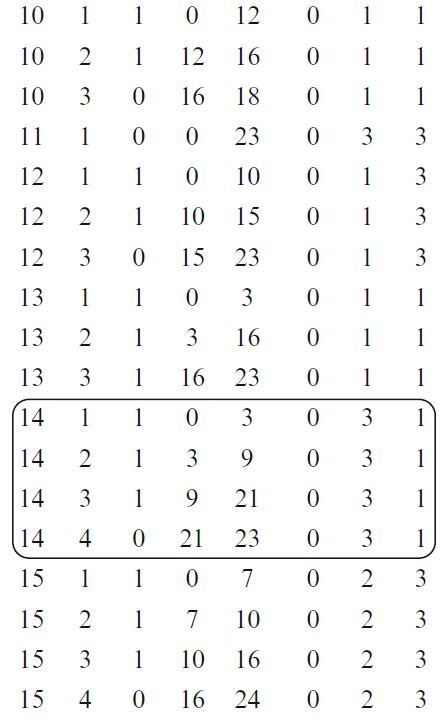
\includegraphics[width =\textwidth, height=5.5cm]{Ch1-CPFormat_2.JPG}
    \end{column}
\end{columns}
\end{block}
\end{frame}

\begin{frame}
\frametitle{Ways to represent (right censored) survival data (cont'd)}
\begin{block}{Fourth way to represent data }
\begin{itemize}
\item This data is the the recurrence of bladder cancer tumors after transurethral surgical excision.
\item Covariates are tx (0 or 1), num and size. Only tx=0 is included here.
\item $i$ is the subject, $j$ is the number of the event for the subject.
\item $d$ is censoring status, \textbf{start} is when event starts, \textbf{stop} is last time of observation of event.
\item For subject 6, two events are observed.
\begin{enumerate}[i.]
\item The first tumor starts at time 0 and stops (excised) at time 6.
\item The second tumor starts at time 6 and the observation is censored at time 10.
\end{enumerate}
\end{itemize}
\end{block}
\end{frame}


\section{Chapter 2}
\begin{frame}
\begin{block}{Problem 2.1}
Given the data below use R to create Kaplan-Kaplan Meirer curves.
\end{block}
\end{frame}

\section{Chapter 7}
\begin{frame}
\begin{block}{Relationships between $S(t), h(t)$ and $f(t)$}
\begin{align*}
& S(t) = P(T>t) = \int_t^\infty f(u) du  \\
& h(t) = \dfrac{-d[S(t)]/dt}{S(t)} \\
& S(t) = \exp\left(-\int_0^t h(u)\right) \\
& f(t) = h(t) S(t)
\end{align*}
$H(u)=\int_0^t h(u)$ is known as the \textbf{cumulative hazard function}.
\end{block}
\end{frame}
\begin{frame}
\begin{block}{Definition 7.1 - Three properties of survival analysis populations}
Let $X$ and $X^*$ be any two different specifications of the covariates.
\begin{enumerate}
\item Proportional Hazards (PH)
\[ h(t;X)/h(t;X^*) = \theta \text{ for all } t>0, \text{ constant } \theta > 0 \]
\item Accelerated Failure Times (AFT)
\[ S(t;X) =  S(\gamma t;X^*)  \text{ for all } t>0, \text{ constant } \gamma > 0
\]
\item Proportional Odds (PO)
\[ \frac{1- S(t;X)}{S(t;X)} = \tau \left(\frac{1- S(t;X^*)}{S(t;X^*)}\right)  \text{ for all } t>0, \text{ constant } \tau > 0
\]
\end{enumerate}
\end{block}
\end{frame}

\begin{frame}
\begin{block}{Three popular parametric distributions}
\begin{center}
\begin{tabular}{ c c c | c }
Distribution & $S(t)$ & $h(t)$ & Accommodates \\ \hline
Exponential & $\exp(\lambda t)$ & $\lambda$ & PH, AFT \\
Weibull  & $\exp(-\lambda t^p)$ & $\lambda p t^{p-1}$ & PH, AFT\\
Log-logistic & $\frac{1}{1+\lambda t^p}$ & $ \frac{\lambda p t^{p-1}}{1+\lambda t^p}$ & PO, AFT
\end{tabular}
\end{center}
\end{block}
\end{frame}

\begin{frame}{Example 7.2 - Modeling Remission Data w/Exponential Model}
\begin{block}{Remission Data} 
\begin{enumerate}[ ]
\item Remission data ($n=42$). Covariate treatment status (TR).
\item 21 given treatment (TR=1). 21 given placebo (TR=0).
\end{enumerate}
\end{block} 
\begin{block}{As a PH model} 
Assuming an exponential distribution, we parameterize 
\[ h(t;TR)= \lambda = \exp(\beta_0 + \beta_1 TRT)
\]
We have hazard ratio
\[
\text{ HR(TR=0 vs. TR=1) } = \exp(\beta_1 \text{TR})
\]
 \end{block}
 \end{frame}
 
 \begin{frame}{Example 7.2 - Modeling Remission Data w/Exponential Model, cont'd}

\begin{block}{As a AFT model}
Assuming an exponential distribution, we parameterize
\[ \frac{1}{\lambda} = \exp(\alpha_0 + \alpha_1 TRT)
\]
We have AF factor
\[
\text{ AF(TR=0 vs. TR=1) } = \exp(\alpha_1 \text{TR})
\]
 \end{block}
 \end{frame}

\end{document} 